\chapter{Introdução}
\label{cap:introducao}

\section{Contextualização e Cenário dos Jogos Digitais}
\label{sec:contextualizacao}

A indústria global de jogos digitais consolidou-se nas últimas décadas como um dos segmentos mais dinâmicos e lucrativos do entretenimento contemporâneo. De acordo com o relatório econômico da Newzoo \cite{newzoo2024games}, o mercado global de jogos movimentou aproximadamente 187,7 bilhões de dólares em 2024, alcançando uma audiência estimada em 3,42 bilhões de jogadores ativos no planeta. Esse volume financeiro supera expressivamente o faturamento anual somado das indústrias de cinema em bilheteria e música gravada, consolidando os jogos como a principal mídia interativa da cultura digital.

Paralelamente a essa massiva expansão de mercado, as expectativas do público consumidor por experiências mais profundas, mundos virtuais críveis e narrativas não lineares cresceram em ritmo acelerado. No entanto, para atender a essa demanda por sofisticação estética e dramática, a produção de títulos de grande escala (frequentemente denominados produções AAA) passou a exigir ciclos de desenvolvimento que rotineiramente ultrapassam cinco a oito anos, mobilizando equipes multidisciplinares com centenas de profissionais e orçamentos multimilionários \cite{schreier2017blood}.

A inflação dos custos de produção atingiu patamares críticos na indústria contemporânea. No início dos anos 2000, títulos de grande sucesso eram concluídos com orçamentos situados entre 10 e 25 milhões de dólares. Em contraste, produções recentes registram cifras alarmantes: a desenvolvedora polonesa CD Projekt Red divulgou oficialmente que o título \textit{Cyberpunk 2077} consumiu cerca de 316 milhões de dólares até o seu lançamento (174 milhões em desenvolvimento direto e 142 milhões em campanhas de marketing), ultrapassando a marca de 440 milhões de dólares de investimento total ao se contabilizarem as reformulações técnicas e a expansão \textit{Phantom Liberty} \cite{cdprojekt2023report}. De forma análoga, documentos corporativos da Sony e da Insomniac Games revelaram que o título \textit{Marvel's Spider-Man 2} exigiu mais de 315 milhões de dólares de orçamento, enquanto \textit{The Last of Us Part II}, da Naughty Dog, ultrapassou 220 milhões de dólares em custos diretos de engenharia e arte.

\begin{figure}[htbp]
\centering

\includegraphics[width=0.78\textwidth]{figuras/dialogue_cyberpunk.jpg}
\caption{Interface contemporânea de diálogo em produções AAA (exemplo em \textit{Cyberpunk 2077}), evidenciando a mecânica de seleção manual de opções pré-definidas.}
\label{fig:cyberpunk_dialogo}
\end{figure}

Apesar desses investimentos monumentais, a forma fundamental como os jogadores interagem verbalmente com os habitantes desses mundos virtuais permanece essencialmente a mesma há décadas. Conforme ilustrado na Figura \ref{fig:cyberpunk_dialogo}, mesmo em produções que demandaram centenas de milhões de dólares, o jogador depara-se com uma interface baseada em um menu estático com poucas alternativas de texto pré-escritas.

Historicamente, a interatividade narrativa e o comportamento verbal de Personagens Não Jogáveis (\textit{Non-Player Characters}, NPCs) têm sido estruturados sobre arquiteturas de árvores de diálogo determinísticas e máquinas de estados finitos \cite{adams2014fundamentals}. Embora essas abordagens garantam aos autores e desenvolvedores um controle absoluto sobre a consistência textual e o fluxo da história, elas impõem barreiras intransponíveis à imersão e à agência do jogador. Sob esse paradigma clássico, o jogador é confinado a escolher entre réplicas textuais pré-concebidas; esgotadas as opções do roteiro, o personagem inevitavelmente retorna a ciclos de respostas repetitivas ou declarações genéricas, quebrando a suspensão da descrença \cite{murray1997hamlet}.

\begin{figure}[htbp]
\centering
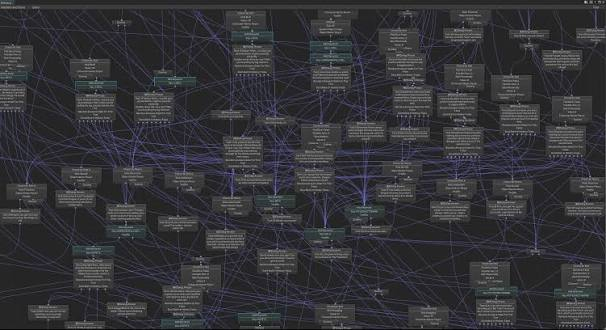
\includegraphics[width=0.82\textwidth]{figuras/arvore_dialogo_complexa.jpg}
\caption{Diagrama de ramificação massiva em uma árvore de diálogo tradicional, ilustrando a complexidade de rastreabilidade de caminhos e a explosão combinatória de autoria.}
\label{fig:arvore_complexa}
\end{figure}

O principal obstáculo intrínseco a essa abordagem de autoria manual é a denominada ``explosão combinatória''. Como exemplificado na Figura \ref{fig:arvore_complexa}, à medida que os roteiristas tentam oferecer ramificações reais de causa e efeito, a árvore de decisões multiplica-se exponencialmente a cada novo diálogo. Rastrear o impacto de centenas de nós interconectados gera um custo de autoria insustentável, forçando os estúdios a convergir os caminhos em nós comuns, resultando em uma sensação frequente de falsa agência ou linearidade disfarçada \cite{riedl2013interactive}.

Nesse cenário de gargalo produtivo, o Processamento de Linguagem Natural (PLN) e a Inteligência Artificial (IA) generativa emergem como alternativas estratégicas para transformar essa realidade. A emergência dos Modelos de Linguagem de Grande Escala (\textit{Large Language Models}, LLMs), fundamentados na arquitetura neural \textit{Transformer} \cite{vaswani2017attention}, viabiliza uma quebra histórica de paradigma. Ao permitirem que o fluxo de desenvolvimento transite da escrita exaustiva de ramificações para a parametrização de personas ricas em contexto \cite{shanahan2023role}, os modelos possibilitam a geração de diálogos em tempo real, nos quais o jogador pode formular perguntas em linguagem natural irrestrita.

\section{Formulação do Problema}
\label{sec:problema}

A superação das árvores estáticas de diálogo por meio de agentes gerativos encontra seu cenário de aplicação mais desafiador no gênero de jogos de mistério e dedução lógica \cite{fernandez2014introduction}. Em um jogo investigativo, a mecânica central (\textit{core gameplay loop}) centraliza-se no inquérito metódico de suspeitos, na coleta de testemunhos e na análise crítica de álibis, distinguindo-se fundamentalmente de dinâmicas baseadas em destreza motora ou combate. A literatura especializada classifica essa dinâmica como ``Linguagem de Processo'' (\textit{Process Language}), um regime interativo no qual o jogador atua como coautor do desdobramento narrativo \cite{fernandez2014introduction}. Para que essa mecânica funcione, o NPC deve sustentar rigorosamente suas restrições de papel, ocultar informações confidenciais de forma coerente e relatar eventos do passado com fidelidade factual inabalável.

No entanto, a inserção de modelos de linguagem generativos em ambientes que demandam determinismo factual revela vulnerabilidades intrínsecas à sua natureza probabilística. Os LLMs operam prevendo o próximo \textit{token} estatisticamente mais provável, o que acarreta o risco persistente de alucinações \cite{ji2023survey}. No contexto de simulação de personas (\textit{roleplay}), essa deficiência manifesta-se criticamente como ``alucinação de personagem'' (\textit{character hallucination}), em que o modelo inventa fatos ausentes do roteiro ou assume posturas contraditórias à sua identidade ficcional.

Em jogos de investigação, o impacto da alucinação de personagem é destrutivo. Se um suspeito afirmar falsamente ter presenciado uma cena em um horário em que se encontrava em outro cômodo, ou revelar detalhes que somente o assassino conheceria, a integridade de todo o mistério é violada. Esse erro de consistência espaço-temporal invalida a dedução lógica do jogador \cite{ahn2024timechara}. Além disso, modelos compactos executados em hardware local sofrem frequentemente do fenômeno de perda de contexto (\textit{Lost in the Middle}) quando submetidos a históricos extensos de conversa \cite{liu2024lost}, ou quebram a persona respondendo de forma metalinguística como assistentes virtuais (\textit{Out-of-Character}, OOC).

\subsection{O Abismo Econômico dos Custos Recorrentes por Token}
\label{subsec:custo_tokens_problema}

Além das vulnerabilidades lógicas, existe uma barreira econômica fundamental que inviabiliza o uso ingênuo de APIs comerciais proprietárias na nuvem (tais como OpenAI GPT-4o ou Anthropic Claude) em jogos de entretenimento comercial.

Os jogos para computadores e consoles são historicamente comercializados sob o modelo de compra única (\textit{Buy-to-Play}, B2P), no qual o consumidor paga um valor fixo (por exemplo, 20 a 70 dólares) e obtém direito irrestrito de jogabilidade por dezenas ou centenas de horas. Nesse modelo de negócios, o estúdio possui receita marginal zero após a venda da cópia. 

Entretanto, as APIs proprietárias de inteligência artificial cobram continuamente por volume de \textit{tokens} trafegados tanto na entrada (\textit{prompt}) quanto na saída (\textit{completion}). Em sessões investigativas densas, onde a cada turno é necessário enviar o histórico de mensagens acumulado, o perfil psicológico e o roteiro do caso, cada requisição consome facilmente entre 3.000 e 6.000 \textit{tokens}. Se um estúdio independente comercializar 50.000 cópias de um jogo e cada jogador realizar uma média modesta de 250 turnos de inquérito ao longo da campanha, o sistema processará mais de 12,5 milhões de chamadas de API, acumulando dezenas de bilhões de \textit{tokens}. Com as tarifas vigentes de modelos de fronteira na nuvem, a fatura de servidores consumiria centenas de milhares de dólares, superando rapidamente a própria margem de lucro líquida obtida com as vendas do jogo. 

Esse descompasso financeiro cria um incentivo perverso inaceitável para o desenvolvedor: quanto mais o jogador se engaja com o jogo e conversa com os personagens, maior é o prejuízo operacional imposto ao estúdio. Portanto, a transição para Modelos Compactos (\textit{Small Language Models}, SLMs) executados diretamente no hardware de borda do usuário final (\textit{edge computing}), com custo marginal estritamente nulo por turno, constitui a única via economicamente sustentável para democratizar NPCs generativos na indústria independente.

\section{Questão de Pesquisa e Hipótese}
\label{sec:questoes_pesquisa}

Diante da problemática exposta, formula-se a seguinte questão norteadora da pesquisa:

\begin{quote}
\textit{Como uma arquitetura híbrida de Agentic RAG com fragmentação temporal dinâmica influencia a consistência espaço-temporal, a fidelidade factual e a estabilidade de persona em NPCs conduzidos por modelos de linguagem compactos executados localmente em jogos de investigação?}
\end{quote}

A hipótese central deste trabalho estabelece que a substituição de \textit{prompts} estáticos completos (\textit{Full Prompt}) por um mecanismo de triagem autônoma (\textit{Agentic RAG}) com fragmentação dinâmica do cronograma factual reduz o ruído informacional na janela de contexto, mitigando alucinações de personagem e permitindo que modelos compactos (entre 7 e 9 bilhões de parâmetros) atinjam níveis satisfatórios de fidelidade factual sem sacrificar a expressividade narrativa da persona, viabilizando economicamente a execução local com custo nulo de infraestrutura em nuvem.

\section{Objetivos}
\label{sec:objetivos}

Para responder à questão norteadora e validar a hipótese proposta, definem-se os seguintes objetivos:

\subsection{Objetivo Geral}
Desenvolver, integrar e avaliar comparativamente uma arquitetura híbrida de \textit{Agentic RAG} com fragmentação temporal dinâmica para a geração em tempo real de diálogos investigativos com NPCs, analisando a consistência espaço-temporal e a resiliência de diferentes modelos de linguagem de porte intermediário executados em ambiente computacional local.

\subsection{Objetivos Específicos}
\begin{enumerate}[label=\roman*.]
    \item Projetar e estruturar o cenário investigativo ficcional e a persona de inquérito (``Alberto Castelo''), formalizando seus atributos em dados estruturados (JSON) segregados em perfil biográfico, cronograma horário e grafo de relacionamentos;
    \item Implementar o ambiente lúdico interativo utilizando o motor gráfico Unity, estabelecendo a comunicação assíncrona com os modelos de linguagem locais gerenciados pela plataforma Ollama através do middleware Neo Cortex;
    \item Conceber e integrar o pipeline de \textit{Agentic RAG} baseado no paradigma ReAct (\textit{Reasoning and Acting}), incorporando o algoritmo de fragmentação dinâmica (\textit{Dynamic Chunking}) para despacho seletivo de blocos horários;
    \item Elaborar uma bateria experimental padronizada de 50 perguntas de inquérito sob estresse, categorizadas em cinco dimensões de vulnerabilidade: filtro de falsa informação, teste de direcionamento, consciência cronológica, resistência a evidências falsas e confronto direto de motivo;
    \item Avaliar quantitativamente o desempenho dos modelos Gemma-2-9b-it, Qwen-2.5-7b, Llama-3.1-8b e DeepSeek-R1-8b por meio do framework RAGAS com juiz sintético GPT-4o, analisando métricas de fidelidade factual, relevância e precisão de recuperação de contexto;
    \item Traçar o perfil comportamental e qualitativo individual de cada arquitetura avaliada, fornecendo diretrizes de engenharia de contexto para desenvolvedores de jogos digitais;
    \item Delinear e formalizar o protocolo experimental de validação ecológica com jogadores humanos na Universidade do Estado do Amazonas (UEA), definindo instrumentos psicométricos (módulo GEQ e escala SUS) para correlacionar a fidelidade computacional com a experiência de imersão e agência do usuário.
\end{enumerate}

\section{Justificativa e Relevância}
\label{sec:justificativa}

A relevância desta pesquisa fundamenta-se em três pilares interconectados:

\begin{itemize}
    \item \textbf{Relevância Científica:} Contribui para a literatura em Processamento de Linguagem Natural aplicada a sistemas interativos, investigando o comportamento de modelos de linguagem abertos em tarefas de simulação sob pressão inquisitiva adversária. Adicionalmente, discute criticamente a adequação de frameworks consolidados de avaliação (RAGAS) quando aplicados ao domínio de dramatização lúdica;
    \item \textbf{Relevância Tecnológica e Econômica:} Demonstra a viabilidade prática da execução de agentes inteligentes autônomos inteiramente em hardware de borda (\textit{edge computing} em computadores pessoais), eliminando as faturas recorrentes de APIs comerciais em nuvem e garantindo soberania de dados, baixa latência e viabilidade financeira definitiva para estúdios independentes;
    \item \textbf{Relevância para a Indústria de Jogos:} Oferece aos designers narrativos uma metodologia concreta de parametrização e controle contextual, reduzindo a complexidade combinatória inerente à autoria de árvores de diálogo sem abrir mão da agência do usuário.
\end{itemize}

\section{Estrutura da Monografia}
\label{sec:estrutura}

A presente monografia encontra-se estruturada em sete capítulos, organizados da seguinte forma:

O \textbf{Capítulo \ref{cap:introducao}} contextualizou o tema com dados econômicos da indústria, delimitou o problema de pesquisa e a barreira financeira de APIs, definiu as hipóteses e enumerou os objetivos gerais e específicos.

O \textbf{Capítulo \ref{cap:referencial}} apresenta o referencial teórico que alicerça o trabalho, discutindo a narrativa interativa em jogos, os fundamentos de LLMs e SLMs, técnicas de RAG e ReAct, as taxonomias de alucinação e os frameworks de avaliação automatizada baseados em LLM-as-a-Judge.

O \textbf{Capítulo \ref{cap:relacionados}} revisa os principais trabalhos relacionados na literatura, comparando abordagens seminais como os Agentes Generativos e estudos de caso comerciais com a proposta desta pesquisa por meio de uma matriz comparativa.

O \textbf{Capítulo \ref{cap:metodologia}} detalha a metodologia de pesquisa baseada no modelo CRISP-DM, a concepção do mistério ficcional e da Fase 1, a taxonomia da bateria de 50 testes de estresse e os protocolos experimental e humano.

O \textbf{Capítulo \ref{cap:implementacao}} documenta a engenharia de software da solução, abordando a integração Unity-NeoCortex-Ollama, os algoritmos de triagem e chunking dinâmico, e a infraestrutura de hardware utilizada.

O \textbf{Capítulo \ref{cap:resultados}} expõe os resultados empíricos, apresentando a análise quantitativa do RAGAS, o desacoplamento entre métricas de recuperação e geração, as transcrições qualitativas de inquérito, as hipóteses para testes humanos e o perfil comparativo dos modelos.

O \textbf{Capítulo \ref{cap:conclusao}} encerra a monografia com as considerações finais, a síntese das contribuições, as limitações metodológicas identificadas e os direcionamentos para trabalhos futuros.
